\documentclass[../main.tex]{subfiles}
\graphicspath{{img},{img/ink},{ink}}

\begin{document}

\begin{tcolorbox}[
    width=\textwidth,
    height=\textheight,
    title=Phyphox: Allgemein,
    fonttitle=\Large,
    before title=\vspace{0.2cm}, after title=\vspace{0.2cm},
    colback=white,
    title filled=true, 
    colbacktitle=myorange,
    colframe=black,
    coltitle=black,
    ]
    \begin{tikzpicture}[remember picture,overlay]
        % Simple brace
        \draw [decorate,
            decoration = {brace,mirror}] (page cs:-0.2,0.585) -- (page cs:-0.2,0.67);
        \draw (page cs:-0.02,0.63) node {jeweils 3 Achsen:};
    \end{tikzpicture}
    \begin{minipage}[]{0.5\textwidth}
        \textbf{Sensoren}: 
        \begin{itemize}[noitemsep]
            \item Beschleunigungessensor
            \item Gyroskop
            \item Magnetfeldsensor
            \item Drucksensor
            \item Lichtsensor (nicht in iOS)
        \end{itemize}
    \end{minipage}
    \hspace{2cm}
    \begin{minipage}[]{0.3\textwidth}
        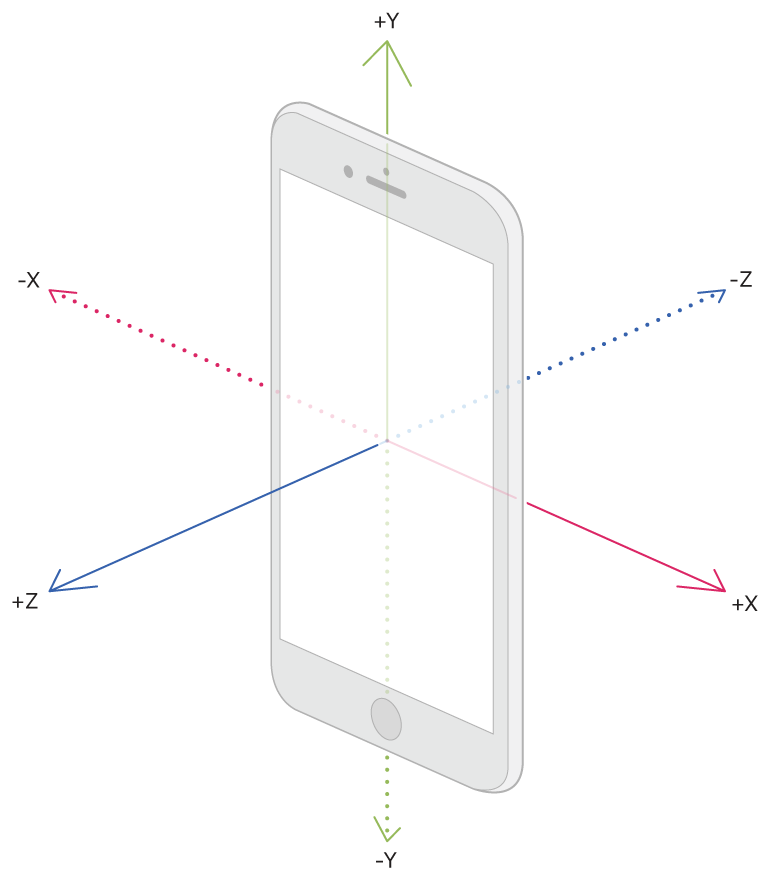
\includegraphics[width=0.8\textwidth]{img/acc}
    \end{minipage}

    \begin{minipage}[]{0.5\textwidth} 
        \textbf{Fernzugriff}: Hat man ein Experiment ausgewählt und drückt auf die 3 Punkte am oberen rechten Eck, lässt sich der \glqq Fernzugriff\grqq{} aktivieren. Die App startet dann einen Server (in der Regel Port 8080) auf dem Gerät und stellt eine Website zur Verfügung, in der die Oberfläche des Experiments gespiegelt und kontrolliert werden kann. Befindet sich ein anderes Gerät im selben Netzwerk wie das Handy, kann über die URL \glqq http://<Ip-Addresse>:<Port>\grqq{} auf diese Website zugegriffen werden.
    \end{minipage}
    \hspace{0.5cm}
    \begin{minipage}[]{0.2\textwidth}
        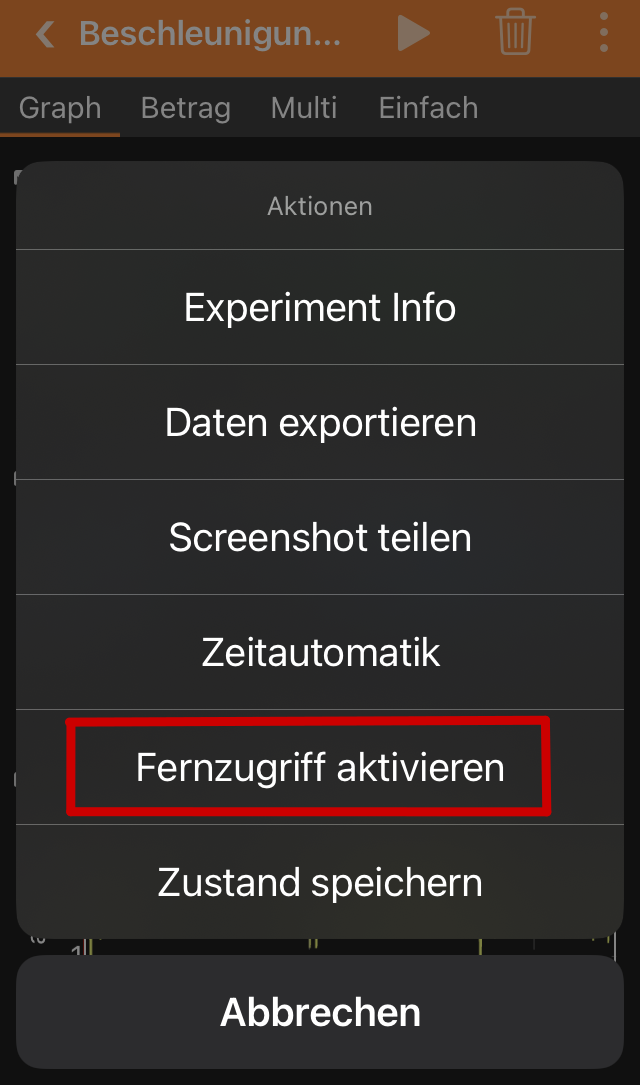
\includegraphics[width=\textwidth]{img/fernzugriff2}
    \end{minipage}
    \begin{minipage}[]{0.2\textwidth}
        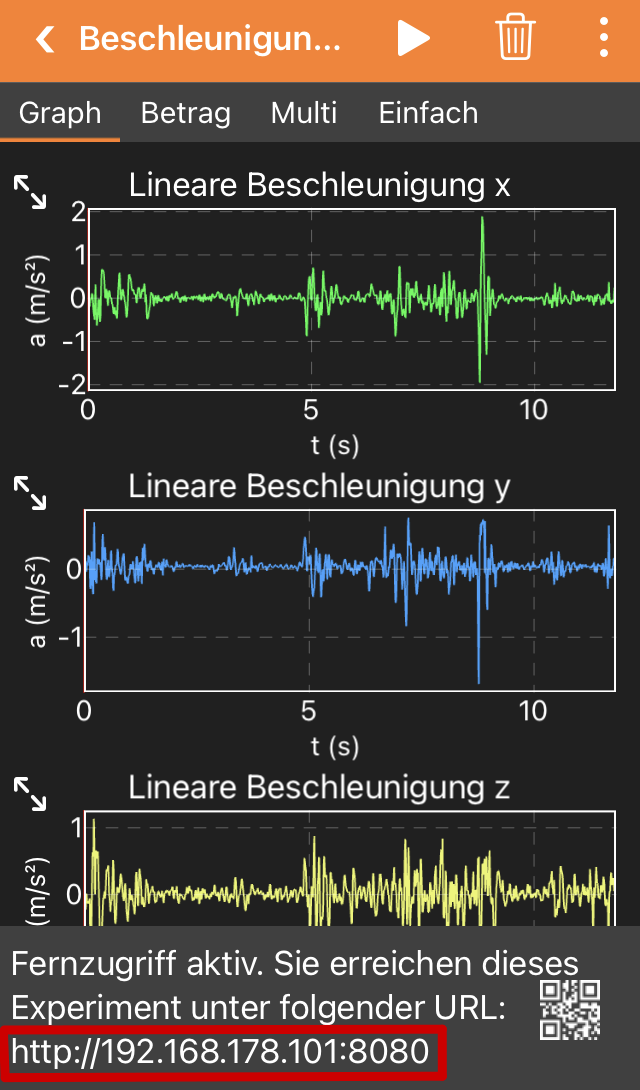
\includegraphics[width=\textwidth]{img/fernzugriff3}
    \end{minipage}
    
    \vspace{0.5cm}
    \textbf{API}: Wird der Fernzugriff gestartet, steht zusätlich eine API zur Verfügung. Durch GET-Methoden lassen sich die Daten der Sensoren anfordern. Damit können z.B. die Daten am Computer in anderer Form aufbereitet werden.  
    
    \vspace{0.5cm}
    \begin{minipage}[]{0.45\textwidth} 
        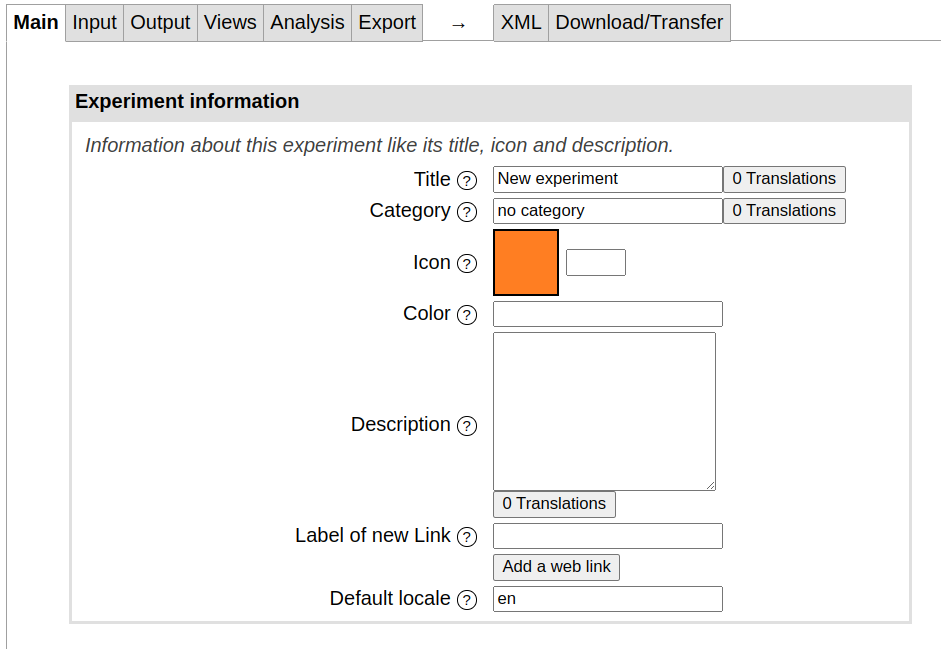
\includegraphics[width=\textwidth]{img/editor}
    \end{minipage}
    \hspace{0.2cm}
    \begin{minipage}[]{0.5\textwidth} 
    \textbf{Eigene Experimente}: Es lassen sich eigene Experimente gestalten. Dazu werden XML-Dateien verwendet. Im Phyphox-Wiki findet man eine ausführliche Erklärung zu den Möglichkeiten (https://phyphox.org/wiki/). Für Anfänger wird von den Entwicklern ein Experiment-Editor bereitgestellt (https://phyphox.org/editor/). Damit lässt sich die XML-Datei des Experiments über grafische Elemente entwickeln. 
    \end{minipage}
    
    \vspace{0.5cm}
    \textbf{Bluetooth Low Energy}: Bei der Gestaltung eigener Experimente lassen sich neben den Sensoren des Handys auch externe Sensordaten einbinden, die über BLE gesendet werden. Neuere Mikrocontroller (Arduino, ESP32, Raspberry Pi) sind in der Regel von Haus aus mit entsprechenden Modulen ausgestattet. Damit lassen sich Daten von externen Sensoren mit den Handysensoren kombinieren und die Darstellungsmöglichkeiten der Phyphox-App nutzen. Man startet dazu einen BLE-Gatt-Server (https://github.com/phyphox/phyphox-arduino) auf dem Mikrocontroller und trägt die Charakteristiken in die XML-Datei eines Experiments ein. Ein solcher Server kann auch dazu dienen um Daten der Handysensoren zu empfangen (Alternative zu GET-Methoden der API).    
\end{tcolorbox}

\end{document}
